%------------------------------------------------------------------------------
% Beginning of journal.tex
%------------------------------------------------------------------------------
%
% AMS-LaTeX version 2 sample file for journals, based on amsart.cls.
%
%        ***     DO NOT USE THIS FILE AS A STARTER.      ***
%        ***  USE THE JOURNAL-SPECIFIC *.TEMPLATE FILE.  ***
%
% Replace amsart by the documentclass for the target journal, e.g., tran-l.
%
\documentclass{amsart}

%     If your article includes graphics, uncomment this command.
\usepackage{graphicx}
\usepackage{comment}
\usepackage{minted}

\newtheorem{theorem}{Theorem}[section]
\newtheorem{lemma}[theorem]{Lemma}

\theoremstyle{definition}
\newtheorem{definition}[theorem]{Definition}
\newtheorem{example}[theorem]{Example}
\newtheorem{xca}[theorem]{Exercise}

\theoremstyle{remark}
\newtheorem{remark}[theorem]{Remark}

\numberwithin{equation}{section}

%    Absolute value notation
\newcommand{\abs}[1]{\lvert#1\rvert}

%    Blank box placeholder for figures (to avoid requiring any
%    particular graphics capabilities for printing this document).
\newcommand{\blankbox}[2]{%
  \parbox{\columnwidth}{\centering
%    Set fboxsep to 0 so that the actual size of the box will match the
%    given measurements more closely.
    \setlength{\fboxsep}{0pt}%
    \fbox{\raisebox{0pt}[#2]{\hspace{#1}}}%
  }%
}

\begin{document}

\title{Project: Wolf Population Management}

%    Information for first author
\author{Jason Hu}
%    Address of record for the research reported here
%\address{Department of Mathematics, Louisiana State University, Baton
%Rouge, Louisiana 70803}
%    Current address
%\curraddr{Department of Mathematics and Statistics,
%Case Western Reserve University, Cleveland, Ohio 43403}
%\email{xyz@math.university.edu}
%    \thanks will become a 1st page footnote.
%\thanks{The first author was supported in part by NSF Grant \#000000.}
%    Information for second author
\author{Qiaqia Ji}
%\address{Mathematical Research Section, School of Mathematical Sciences,
%Australian National University, Canberra ACT 2601, Australia}
%\email{two@maths.univ.edu.au}
%\thanks{Support information for the second author.}

%    General info
%\subjclass[2000]{Primary 54C40, 14E20; Secondary 46E25, 20C20}

%\date{January 1, 2001 and, in revised form, June 22, 2001.}

%\dedicatory{This paper is dedicated to our advisors.}

%\keywords{Differential geometry, algebraic geometry}

\begin{abstract}
We modelled the change of wolf population in a hypothetical habitat under progressively more complicated assumptions, in order to apply our knowledge of ordinary differential equations.
\end{abstract}

\maketitle

%\section*{This is an unnumbered first-level section head}
%This is an example of an unnumbered first-level heading.

%% The correct journal style for \specialsection is all uppercase; a known bug
%% in amsart.cls prevents this, so input must be uppercase until it is fixed.
%\specialsection*{This is a Special Section Head}
%\specialsection*{THIS IS A SPECIAL SECTION HEAD}
%This is an example of a special section head%
%%%%%%%%%%%%%%%%%%%%%%%%%%%%%%%%%%%%%%%%%%%%%%%%%%%%%%%%%%%%%%%%%%%%%%%%
%\footnote{Here is an example of a footnote. Notice that this footnote
%text is running on so that it can stand as an example of how a footnote
%with separate paragraphs should be written.
%\par
%And here is the beginning of the second paragraph.}%
%%%%%%%%%%%%%%%%%%%%%%%%%%%%%%%%%%%%%%%%%%%%%%%%%%%%%%%%%%%%%%%%%%%%%%%%

\section{Without harvesting penalty}

\subsection{Substitutions for K and M}

To find out the expression for K, the carrying capacity of the habitat, notice that wolf population decreases when its density exceeds 1 pack per 25 square miles, and vice versa. Knowing that a pack constitutes 10 wolves on average and the habitat occupies A square miles, it can be inferred that

\begin{equation}
    K = \frac{10A}{25}=\frac{2A}{5}.
\end{equation}

Similarly, to find out the expression for M, the critical minimum population, notice that the wolf population will decline when the density dips below 1 wolf per 25 square miles. It can be inferred that
\begin{equation}
    M=\frac{A}{25}.
\end{equation}

Given the original differential equation
\begin{equation}
    \frac{dN}{dt}=rN(1-\frac{N}{K})(\frac{N}{M}-1),
\end{equation}
we can substitute (1.3) with (1.1) and (1.2), so we have
\begin{equation}
    \frac{dN}{dt}=rN(1-\frac{5N}{2A})(\frac{25N}{A}-1).
\end{equation}

\subsection{Classification of differential equation}

As we can see in Equation (1.4), on the left side is a first derivative of population over time, whereas on the right side, the dependent variable $N$ is multiplied three times. Also, it is obvious that the independent variable $t$ does not show up in (1.4). Thus we can conclude that the ODE is first-order, nonlinear, and autonomous.


In order to find the equilibrium solutions, let equation (1.4) be zero:
\begin{equation}
    \frac{dN}{dt}=rN(1-\frac{5N}{2A})(\frac{25N}{A}-1)=0
\end{equation}

The three roots we get are $N=0$, $N=M=\frac{A}{25}$, and $N=K=\frac{2A}{5}$, for any non-specific values of r and A.

\subsection{Plot for N with different initial populations}
Closed form solution to differential equation (1.5) is beyond our knowledge, so we chose to use neumerical methods for approximation, specifically Runge-Kutta method (rk4).

Given parameter values $r=0.02$ and $A=200000$, we can plot $N$ versus $t$ for a wide range of initial population $N_0$, shown in Figure 1.

\begin{figure}[tb]
%\blankbox{.6\columnwidth}{5pc}
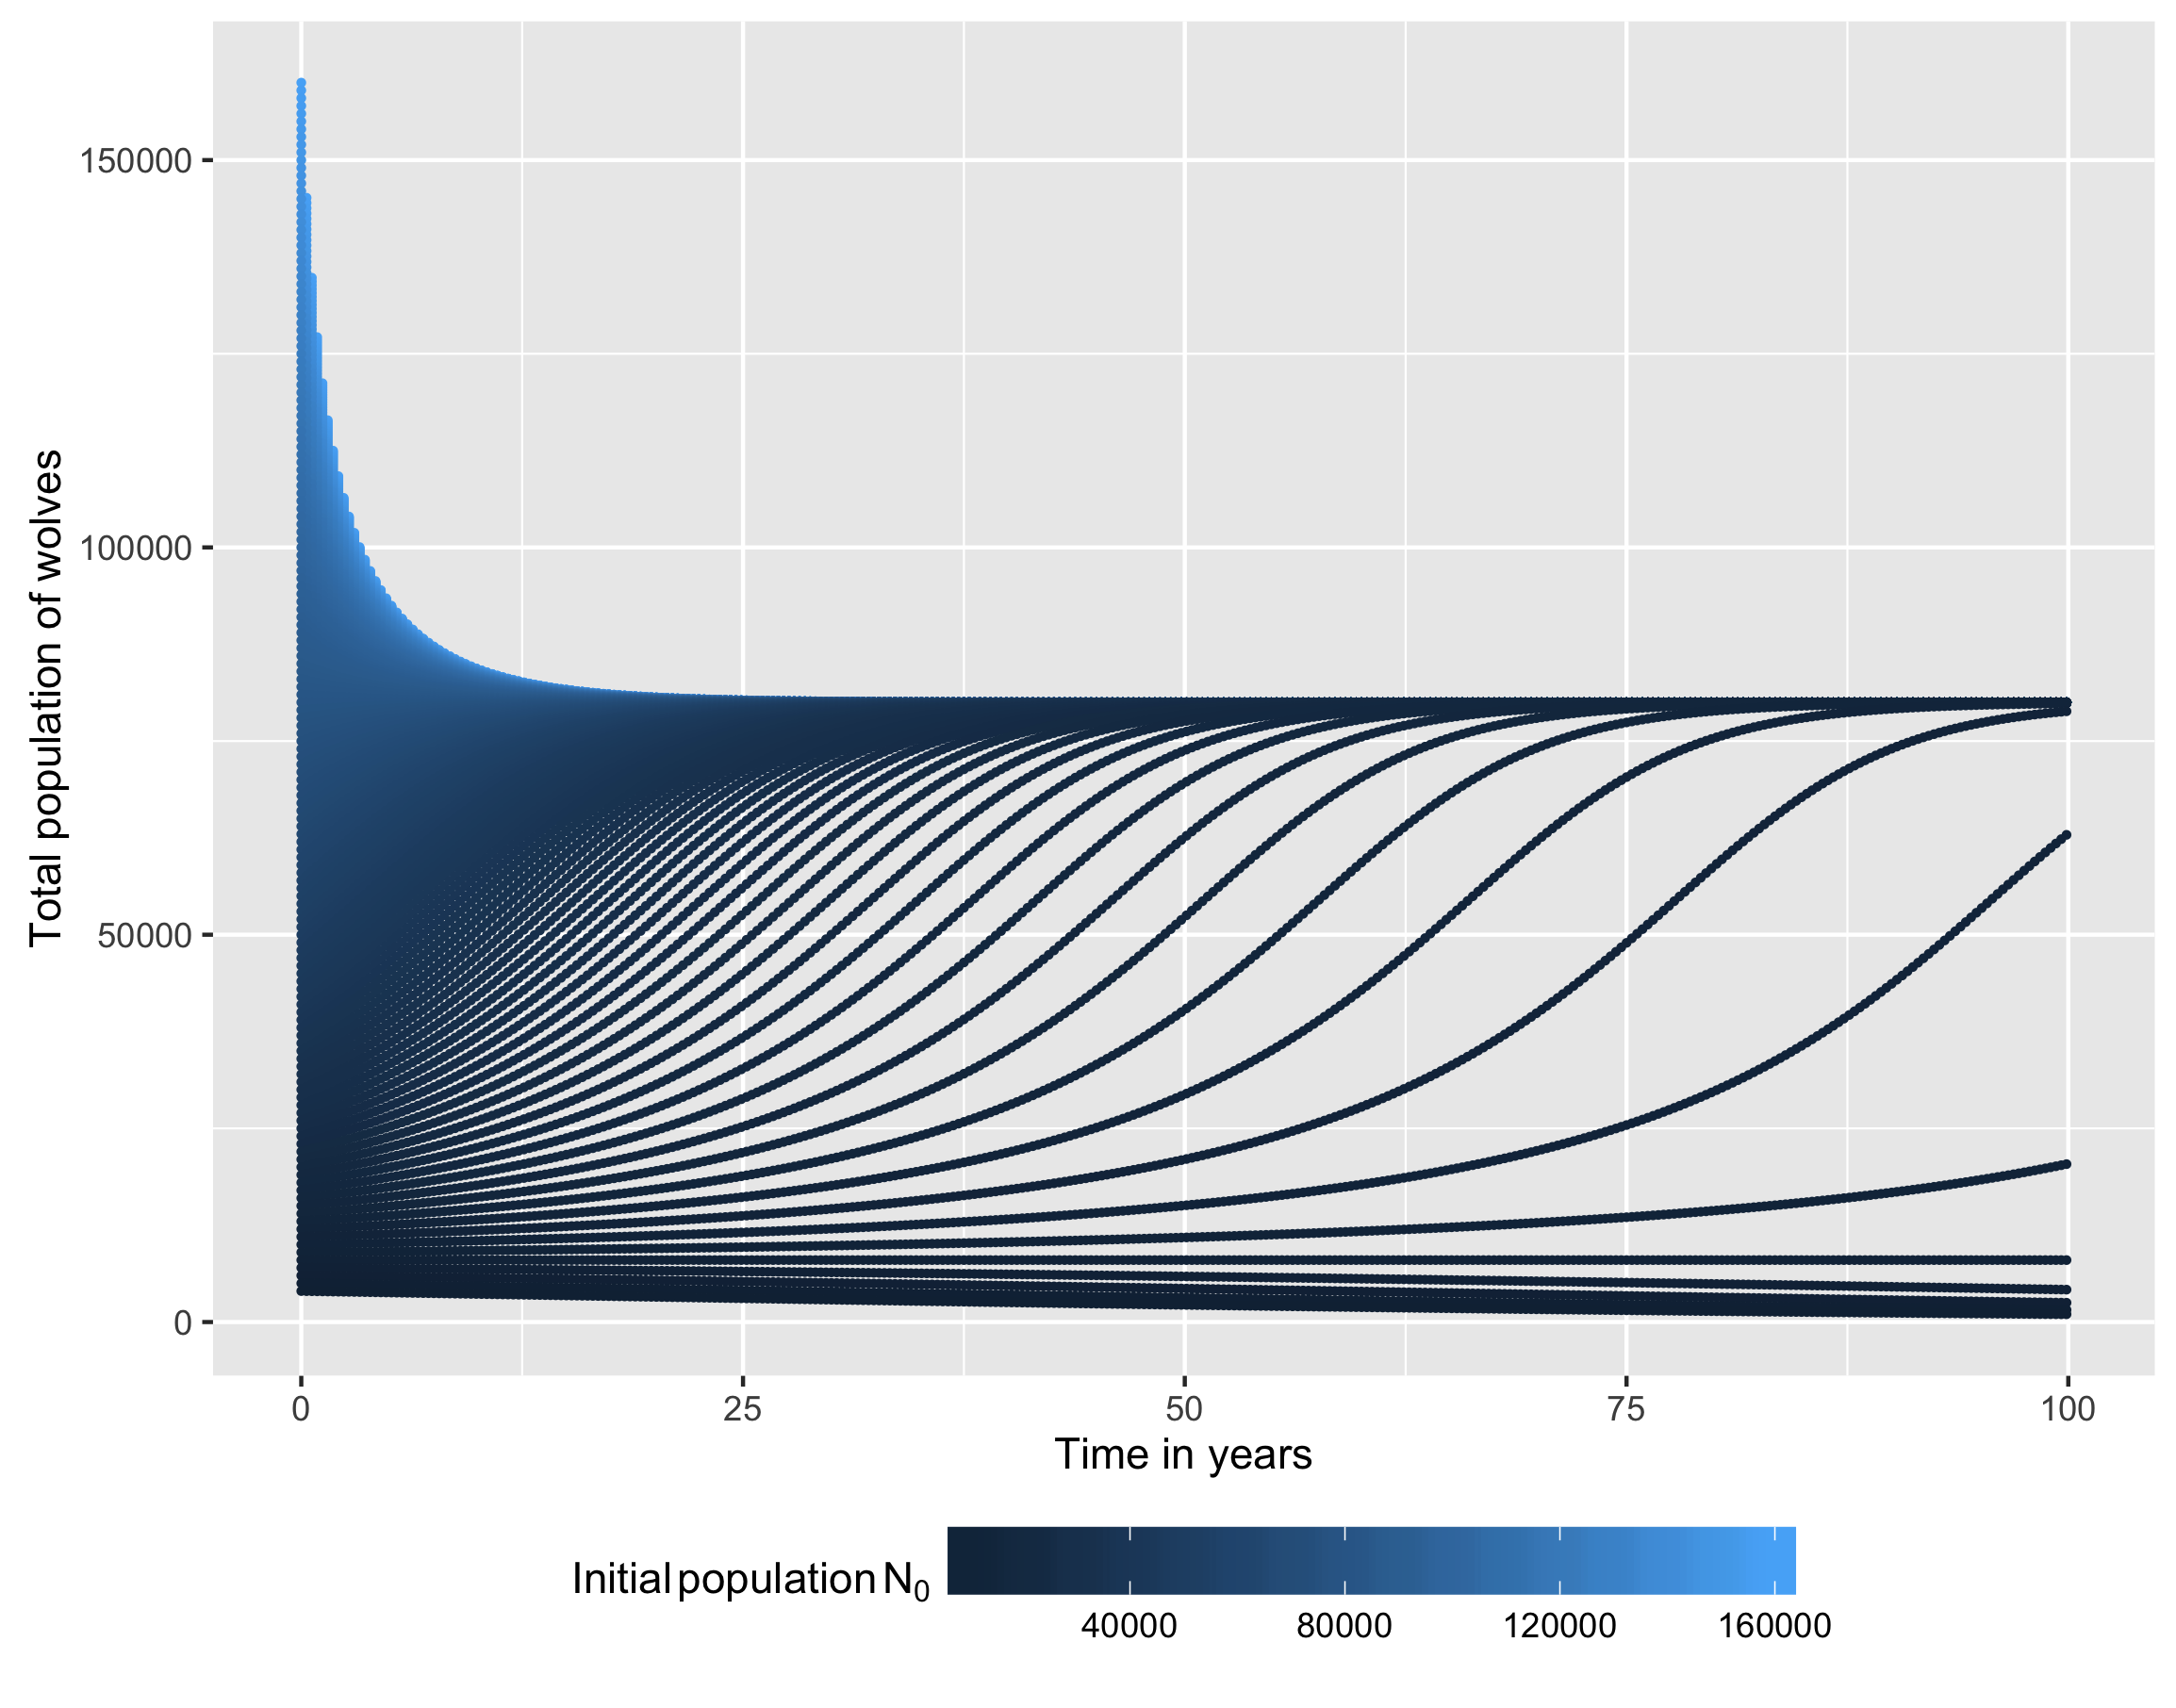
\includegraphics[scale=0.15]{variableN0.png}
\caption{Plot for population $N$ versus $t$, with a range of initial population}
\label{variable}
\end{figure}


\section{With constant harvesting penalty}
\subsection{Qualitative analysis}

Given original differential equation
\begin{equation}
    \frac{dN}{dt}=rN(1-\frac{5N}{2A})(\frac{25N}{A}-1)-h
\end{equation}

To construct the bifurcation diagram, let equation (2.1) be zero and we have
\begin{equation}
    h=rN(1-\frac{5N}{2A})(\frac{25N}{A}-1)
\end{equation}

The solution set ${(h,N)}$ of equation (2.2) is the bifurcation graph. Notice that parameter $h$ is an affine term to the differential equation. It's safe to proclaim that the bifurcation graph should look like a x-y mirror of a third order polynomial.

Equilibrium solutions to original differential equation (2.1) is therefore all the points $(h,N)$ on the bifurcation diagram.

%%%%%%%%%%%%%%%%%%%%%%%%%%%%%%%
\begin{comment}
To find bifurcation values of h, we can solve for all the local extrema $(N^*,h^*)$ for polynomial (2.2), where $h^*$ are all the bifurcation values.
Expand equation (2.2):
\begin{equation}
    h&=-\frac{125rN^3}{2A^2}+\frac{55rN^2}{2A}-rN
\end{equation}

Let the derivative of h (2.3) with regard to N be zero:
\begin{equation}
    \frac{dh}{dN}&=-\frac{375rN^2}{2A^2}+\frac{55rN}{A}-r=0
\end{equation}

Solve equation (2.4), we have
\begin{equation}
 N =\frac{-\frac{55 r}{A}\pm \sqrt{750 A^2 r^2+\frac{3025 r^2}{A^2}}}{375 A^2 r} (A,r \neq0)

\end{equation}
\end{comment}
%%%%%%%%%%%%%%%%%%%%%%%%%%%%%%%%%%%%%%

To find bifurcation values of $h^*$, we can solve for all the local extrema $(N^*,h^*)$ for polynomial (2.2), where $h^*$ are all the bifurcation values. There are two solutions to polynomial (2.2), so there are two bifurcation values.

A rough sketch of the bifurcation diagram is presented in Figure 2. $\frac{dN}{dt}$ is negative in the blue region with downward arrows and is positive in the red region with upward arrows. $h_1$ and $h_2$ are two bifurcation values. K and M are the carrying capacity and minimum population when $h=0$.
\begin{figure}[tb]
%\blankbox{.6\columnwidth}{5pc}
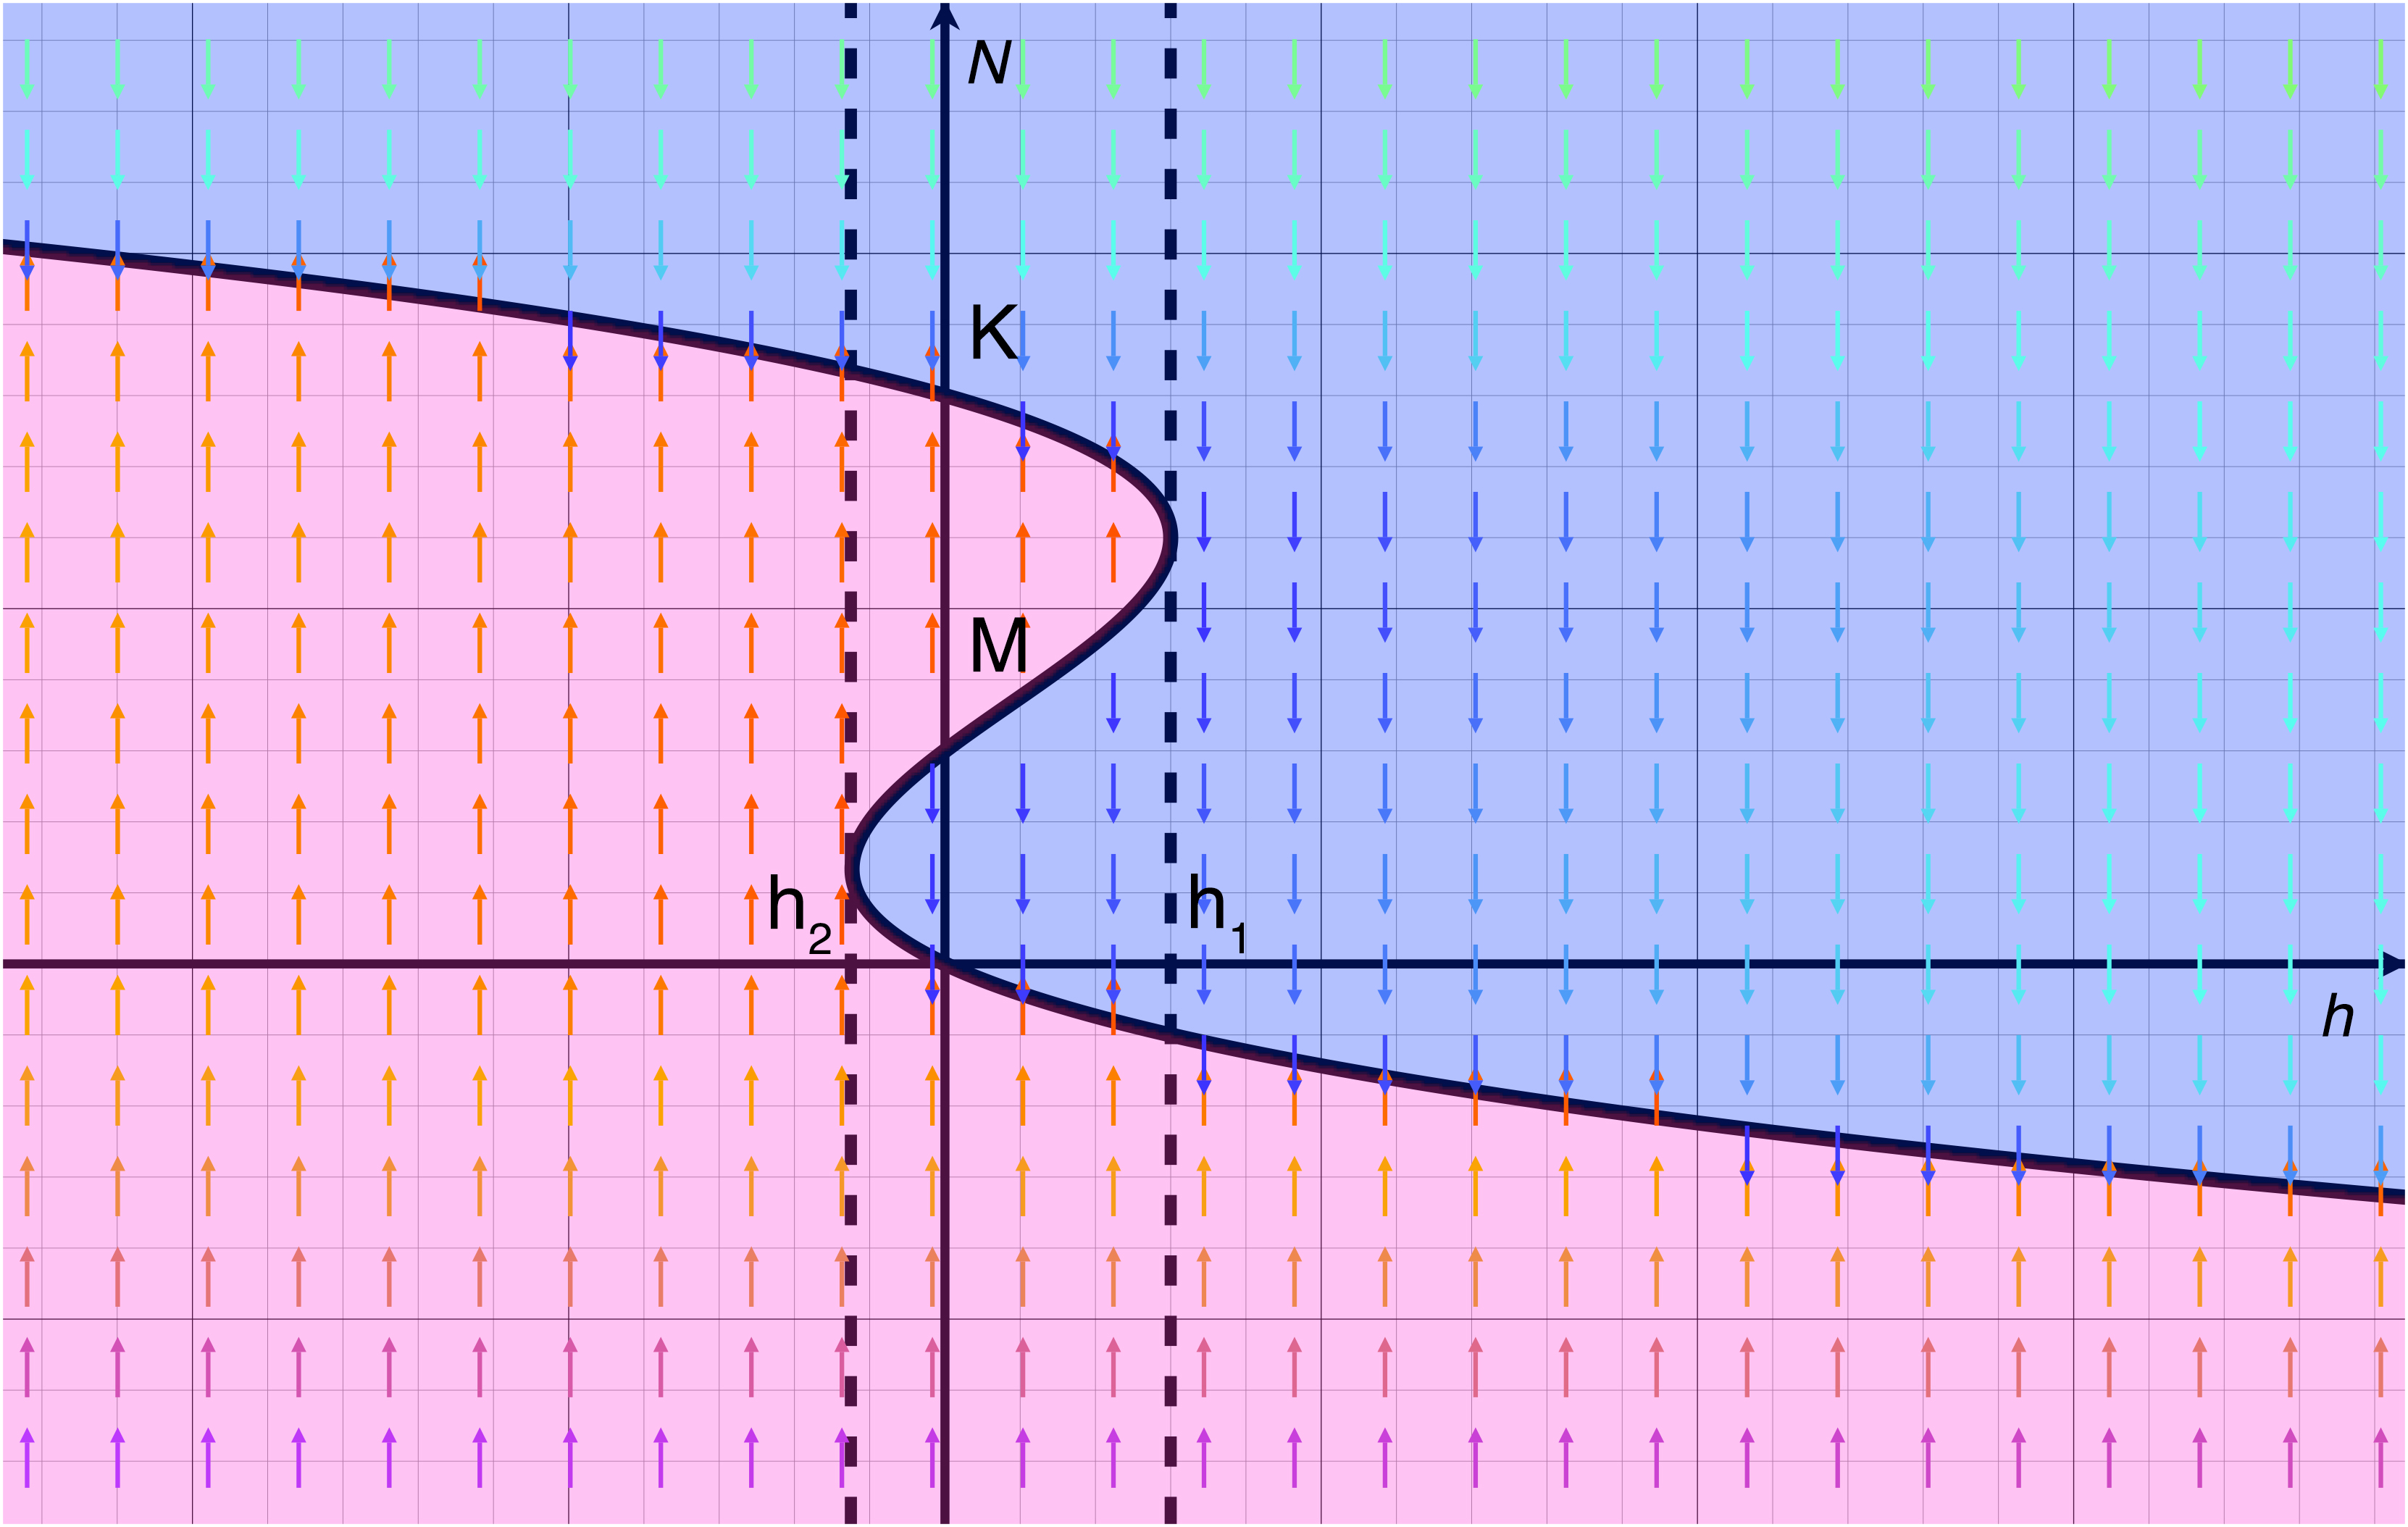
\includegraphics[scale=0.4]{bifurcationdiagram30.jpg}
\caption{Sketch of the bifurcation diagram of the equation (2.1)} SINK? NODE?
\label{variable}
\end{figure}


%%%%%%%%%%%%%%%%%%%%%%%%%%%%%%%
\begin{comment}
Closed form solution to differential equation 2.1 is again beyond our knowledge, so we used Runge-Kutta method to approximate $N(100)$ for different h. To find the maximum $h$ so that $N(100)>0$, note that $N(100)$ can be seen as a function of $h$, and we are looking for a root of function $N_{100}(h)$.

We can use Newton's method to find the root for function $N_{100}(h)$, but first we need to ascertain that there is only one root $h$ for $N(100,h)$. We can prove the monotonicity of $N(100,h)$ as a function of h. 
\end{comment}
%%%%%%%%%%%%%%%%%%%%%%%%%%%%%%%%%%%%%%

%%%%%%%%%%%%%%%%%%%%%%%%%%%%%%
\begin{comment}
Integrate differential equation (2.1) on both sides, and we have
\begin{equation}
\begin{split}
    \int\frac{dN}{dt}dt&=\int \Big(rN(1-\frac{5N}{2A})(\frac{25N}{A}-1)-h\Big) dt \\
    N&=\int rN(1-\frac{5N}{2A})(\frac{25N}{A}-1)dt-\int{hdt}\\
    N&=\int rN(1-\frac{5N}{2A})(\frac{25N}{A}-1)dt-ht
\end{split}
\end{equation}
Population of wolves when $t=100$ can be represented as
\begin{equation}
    N(100,h)=\underbrace{\int^{100}_{0} rN(1-\frac{5N}{2A})(\frac{25N}{A}-1)dt}_\text{constant w.r.t. $h$}-100h
\end{equation}
Note that the integral part in equation (2.4) is constant with regard to h, henceforth $N(100,h)$ is an affine function of h, and it has a unique root.

Given initial population $N(0)=1.5K=120000$, we can use Runge-Kutta method again to approximate numerically the value of the integral in expression (2.4). We selected a time step of 0.2, which leads to 500 time steps in total from 0 to 100. Part of the results are presented in Table 1.


\begin{table}[ht]
\caption{Runge Kutta results for $N_0=120000$}\label{RungeKutta}
\renewcommand\arraystretch{1.5}
\noindent\[
\begin{array}{|c|c|c|}
\hline
\text{Time step}&t&N\\
\hline
0&0&1200000\\
\hline
50&10&99774.80\\
\hline
100&20&91769.29\\
\hline
150&30&87553.68\\
\hline
200&40&85044.47\\
\hline
250&50&83449.02\\
\hline
300&60&82393.57\\
\hline
350&70&81677.50\\
\hline
400&80&81183.49\\
\hline
450&90&80838.79\\
\hline
500&100&80596.38\\
\hline
\end{array}
\]
\end{table}


To find the maximum h, let expression (2.4) be zero:
\begin{equation}
    N(100,h)=\int^{100}_0 rN(1-\frac{5N}{2A})(\frac{25N}{A}-1)dt-100h=0
\end{equation}
Substitute the result from Runge-Kutta approximation into (2.5), we have
\begin{equation}
\begin{split}
    100h&=80596.38\\
    h&\approx805
\end{split}
\end{equation}
That is, 805 wolves per year is the maximum harvesting rate that does not cause the wolf population to be depleted in 100 years.

\end{comment}
%%%%%%%%%%%%%%%%%%%%%%%%%%%%%%%

%%%%%%%%%%%%%%%%%%%%%%%%%%%%%%
\begin{comment}

 Note that $\frac{dN}{dt}$ is continuous on both N and h. Suppose that when $h=h_1$, $N$ reaches equilibrium point $N^*$ for some $t^*<100$. By continuity of $\frac{dN}{dt}$ on h, we have 
\begin{equation}
    \lim_{h\to h_1^+}\frac{dN(t^*,h)}{dt}=\frac{dN(t^*,h_1)}{dt}=0
\end{equation}
And by continuity of $\frac{dN}{dt}$ on N, we have
\begin{equation}
    \lim_{h\to h_1^+}N(100,h)=N(100,h^*)=N^*
\end{equation}
By reading bifurcation diagram Figure 2, we know that as $h$ increases from $h_1$, $\frac{dN}{dt}$ is negative and will monotonically and continuously decrease for any given $N$, we can infer that  $N(100,h)$ will monotonically decrease for $h$ and therefore has only one root for $h$. $N(100,h)$ will decrease from $N^*$ as $h$ increases, until it reaches an equilibrium point, which is negative and practically should be treated as zero.

We can use Newton's method to find the root for function $N_{100}(h)$, but first we need to ascertain that there is only one root $h$ for $N(100,h)$. Note that $\frac{dN}{dt}$ is continuous on both N and h. Suppose that for some $h^*\in(h_1-\sigma_1,h_1)$ for small $\sigma_1$, $N$ reaches equilibrium point $N^*$ for some $t^*<100$. As $h$ continuously increases to $(h_1,h_1+\sigma_1)$ for small $\sigma_1$, the derivative $N(t)$ at time $t=t^*$ suffices
$0<\frac{dN(t^*,h)}{dt}<\sigma_2$ for some small $\sigma_2$, and  $0<N^*-N(100,h)<\sigma_3$ for some small $\sigma_3$
\end{comment}
\begin{comment}
Note that $\frac{dN}{dt}$ (2.1) is a autonomous differential equation. Looking at Figure 2, we know that for a fixed value of positive $h$, $N$ decreases in the neighbourhood of $N=0$, therefore $N(t)=0$ only has one solution $t$. for  The R code used is supplied in Appendix I. Search steps and results are presented in table 1.
\end{comment}
%%%%%%%%%%%%%%%%%%%%%%%%%%%%%%%%


\subsection{Search for the maximum $h$ that preserves wolves in 100 years} 

Closed form solution to differential equation 2.1 is again beyond our knowledge, so we used Runge-Kutta method to approximate $N(100)$ for different h. To find the maximum $h$ so that $N(100)>0$, note that $N(100)$ can be seen as a function of $h$, and we are looking for a root of function $N(100,h)$.

We can use some optimization scheme to find the root for function $N(100,h)$, but first we need to convince ourselves that there is only one root $h$ for $N(100,h)$. Note that $\frac{dN}{dt}$ is continuous on $N$ and $h$, and $\frac{dN}{dt}$ is negative for $N>0, h>h_1$. For a given initial population $N_0$, as $h$ continuously increases, $N(100,h)$ continuously decreases to the equilibrium point.

Given initial population $N(0)=120000>K$, we know that a root $h$ for $N(100,h)=0$ exists only when $h>h_1$, where $N(100,h)$ monotonically decreases as stated above. We conclude that there exists one and only one root $h$ for $N(100,h)=0$.

To search for maximal $h$ such that $N(100,h)>0$, it's possible to modify Runge-Kutta methods for a computationally efficient algorithm. But here we decided to use brute force instead. We relied on Runge-Kutta method to calculate $N(100,h)$ for every given h. We optimized h simply using binary search. Suppose we start with $h=10000$ and aim for a one-decimal-place precision, given that $\log_2 10000\approx16.6$, the optimization is feasible. Results of the optimization is presented in Table 1.

% latex table generated in R 3.2.4 by xtable 1.8-2 package
% 
\begin{table}[ht]
\caption{}\label{eqtable}
\renewcommand\arraystretch{1.5}
\noindent\[
\begin{array}{|c|c|c|}
  \hline
 & h & N(100,h) \\ 
  \hline
1 & 5000.00 & -33721.89 \\ \hline
  2 & 2500.00 & -22556.96 \\ \hline
  3 & 1250.00 & 71078.98 \\ \hline
  4 & 1875.00 & 62375.55 \\ \hline
  5 & 2187.50 & 47968.03 \\ \hline
  6 & 2343.75 & 9102.03 \\ \hline
  7 & 2421.88 & -15772.75 \\ \hline
  8 & 2382.81 & -5957.67 \\ \hline
  9 & 2363.28 & 1154.78 \\ \hline
  10 & 2373.05 & -2553.67 \\ \hline
  11 & 2368.16 & -732.39 \\ \hline
  12 & 2365.72 & 203.70 \\ \hline
  13 & 2366.94 & -266.32 \\ \hline
  14 & 2366.33 & -31.79 \\ \hline
  15 & 2366.03 & 85.83 \\ \hline
  16 & 2366.18 & 26.99 \\ \hline
  17 & 2366.26 & -2.41 \\
   \hline
\end{array}
\]
\end{table}

Our optimization shows that the maximal harvest rate is $h\approx2366.2$ wolves per year such that the wolf population does not deplete in 100 years.


\section{Environmental threat and harvesting scheme}
\subsection{Differential equation with human encroachment and climate fluctuations} We can model the proportional decrease of habitat with expression

\begin{equation}
    A(t)=A_0d^t.
\end{equation}
Consequently, M and K are changed due to dependence on A:
\begin{equation}
    M(t)=\frac{A}{25}=\frac{A_0d^t}{25},
\end{equation}
\begin{equation}
    K(t)=\frac{2A}{5}=\frac{2A_0d^t}{5}.
\end{equation}
Furthermore, we can model the impact of climate fluctuation with expression
\begin{equation}
    K(t)=\frac{10A_0d^t}{-\frac{75}{2}\cos(\frac{\pi}{11}t)+\frac{125}{2}}=\frac{4A_0d^t}{-15\cos(\frac{\pi}{11}t)+25}.
\end{equation}
So we can modify the original differential equation (2.1) to be
\begin{equation}
    \frac{dN}{dt}=rN(1+\frac{15N\cos(\frac{\pi}{11}t)-25N}{4A_0d^t})(\frac{25N}{A_0d^t}-1)-h
\end{equation}
\subsection{Search for maximal harvesting rate $h$ under harsher conditions} Again we will use Runge-Kutta method combined with binary search, to a precision of one decimal place. We have assumed the parameter for encroachment proportion per year $d=0.99$. The optimization results are presented in Table 2.

% latex table generated in R 3.2.4 by xtable 1.8-2 package
% 
\begin{table}[ht]
\caption{}\label{eqtable}
\renewcommand\arraystretch{1.5}
\noindent\[
\begin{array}{|c|c|c|}
    \hline
  & h & N(100,h) \\ \hline
 1 & 5000.00 & -14516.73 \\ 
   \hline
2 & 2500.00 & -11063.22 \\ 
   \hline
3 & 1250.00 & -8382.14 \\ 
   \hline
4 & 625.00 & -6208.68 \\ 
   \hline
5 & 312.50 & 6982.19 \\ 
   \hline
6 & 468.75 & -3927.95 \\ 
   \hline
7 & 390.62 & 1534.07 \\ 
   \hline
8 & 429.69 & -1706.57 \\ 
   \hline
9 & 410.16 & -159.06 \\ 
   \hline
10 & 400.39 & 680.42 \\ 
   \hline
11 & 405.27 & 257.43 \\ 
   \hline
12 & 407.71 & 48.19 \\ 
   \hline
13 & 408.94 & -55.70 \\ 
   \hline
14 & 408.33 & -3.82 \\ 
   \hline
\end{array}
\]
\end{table}

As a result, the maximum rate of harvest under harsh environmental constraints is smaller than that without, which is about $h\approx 408.2$ wolves per year.

\subsection{Design of variable harvesting scheme} We are asked to maintain the wolf population to be $N_{target}\approx40000$, that is, when $N=N_{target}$, it's ideal that $\frac{dn}{dt}=0$.
Substitute this condition into expression (3.5) and eliminate parameters, we have
\begin{equation}
    \frac{dN}{dt}=0.02\cdot40000(1+\frac{15\cdot40000\cos(\frac{\pi}{11}t)-25\cdot40000}{4\cdot 200000d^t})(\frac{25\cdot40000}{200000d^t}-1)-h.
\end{equation}
Assume that $d=0.99$, let expression (3.6) be zero, we have:
\begin{equation}
    h(t)=800(1+\frac{3\cos(\frac{\pi}{11}t)-5}{4\cdot 0.99^t})(\frac{5}{0.99^t}-1)
\end{equation}

Expression (3.7) represents the harvest scheme that will eventually maintain wolf population to be 40000, if it ever reaches there. We can use Runge-Kutta methods to verify this solution. The approximation process is charted in Table 3, and the plot of population against time is provided in Figure 3.

We can see that indeed the population was indeed maintained at 40000, and the population was less variable compared to that under no harvesting scheme.


\begin{table}[ht]
\caption{}\label{eqtable}
\renewcommand\arraystretch{1.5}
\noindent\[
\begin{array}{|c|c|c|}
 \hline
  \text{Time Step}& \text{Time} & N(t) \\ 
  \hline
 0 & 0& 120000.00 \\ 
   \hline
20 & 4& 72721.74 \\ 
   \hline
40 & 8& 47459.88 \\ 
   \hline
60 & 12& 41137.40 \\ 
   \hline
80 & 16& 40231.04 \\ 
   \hline
100 & 20& 40129.27 \\ 
   \hline
120 & 24& 40131.29 \\ 
   \hline
140 & 28& 40059.65 \\ 
   \hline
160 & 32& 40005.41 \\ 
   \hline
\end{array}
\]
\end{table}


\begin{figure}[h]
%\blankbox{.6\columnwidth}{5pc}
\includegraphics[scale=0.15]{hello.png}
\caption{Plot for population change under two harvesting schemes}
\label{HarvestingSchemes}
\end{figure}

%%%%%%%%%%%%%%%%%%%%%%%%%%%%%%%%%%%%%%%%%%%%
\begin{comment}
\subsection*{**************************}
This is an example of an unnumbered second-level heading.

\subsubsection{This is a numbered third-level section head}
This is an example of a numbered third-level heading.

\subsubsection*{This is an unnumbered third-level section head}
This is an example of an unnumbered third-level heading.

\begin{lemma}
Let $f, g\in  A(X)$ and let $E$, $F$ be cozero
sets in $X$.
\begin{enumerate}
\item If $f$ is $E$-regular and $F\subseteq E$, then $f$ is $F$-regular.

\item If $f$ is $E$-regular and $F$-regular, then $f$ is $E\cup
F$-regular.

\item If $f(x)\ge c>0$ for all $x\in E$, then $f$ is $E$-regular.

\end{enumerate}
\end{lemma}

The following is an example of a proof.

\begin{proof} Set $j(\nu)=\max(I\backslash a(\nu))-1$. Then we have
\[
\sum_{i\notin a(\nu)}t_i\sim t_{j(\nu)+1}
  =\prod^{j(\nu)}_{j=0}(t_{j+1}/t_j).
\]
Hence we have
\begin{equation}
\begin{split}
\prod_\nu\biggl(\sum_{i\notin
  a(\nu)}t_i\biggr)^{\abs{a(\nu-1)}-\abs{a(\nu)}}
&\sim\prod_\nu\prod^{j(\nu)}_{j=0}
  (t_{j+1}/t_j)^{\abs{a(\nu-1)}-\abs{a(\nu)}}\\
&=\prod_{j\ge 0}(t_{j+1}/t_j)^{
  \sum_{j(\nu)\ge j}(\abs{a(\nu-1)}-\abs{a(\nu)})}.
\end{split}
\end{equation}
By definition, we have $a(\nu(j))\supset c(j)$. Hence, $\abs{c(j)}=n-j$
implies (5.4). If $c(j)\notin a$, $a(\nu(j))c(j)$ and hence
we have (5.5).
\end{proof}

\begin{quotation}
This is an example of an `extract'. The magnetization $M_0$ of the Ising
model is related to the local state probability $P(a):M_0=P(1)-P(-1)$.
The equivalences are shown in Table~\ref{eqtable}.
\end{quotation}

\begin{table}[ht]
\caption{}\label{eqtable}
\renewcommand\arraystretch{1.5}
\noindent\[
\begin{array}{|c|c|c|}
\hline
&{-\infty}&{+\infty}\\
\hline
{f_+(x,k)}&e^{\sqrt{-1}kx}+s_{12}(k)e^{-\sqrt{-1}kx}&s_{11}(k)e^
{\sqrt{-1}kx}\\
\hline
{f_-(x,k)}&s_{22}(k)e^{-\sqrt{-1}kx}&e^{-\sqrt{-1}kx}+s_{21}(k)e^{\sqrt
{-1}kx}\\
\hline
\end{array}
\]
\end{table}

\begin{definition}
This is an example of a `definition' element.
For $f\in A(X)$, we define
\begin{equation}
\mathcal{Z} (f)=\{E\in Z[X]: \text{$f$ is $E^c$-regular}\}.
\end{equation}
\end{definition}

\begin{remark}
This is an example of a `remark' element.
For $f\in A(X)$, we define
\begin{equation}
\mathcal{Z} (f)=\{E\in Z[X]: \text{$f$ is $E^c$-regular}\}.
\end{equation}
\end{remark}

\begin{example}
This is an example of an `example' element.
For $f\in A(X)$, we define
\begin{equation}
\mathcal{Z} (f)=\{E\in Z[X]: \text{$f$ is $E^c$-regular}\}.
\end{equation}
\end{example}

\begin{xca}
This is an example of the \texttt{xca} environment. This environment is
used for exercises which occur within a section.
\end{xca}

The following is an example of a numbered list.

\begin{enumerate}
\item First item.
In the case where in $G$ there is a sequence of subgroups
\[
G = G_0, G_1, G_2, \dots, G_k = e
\]
such that each is an invariant subgroup of $G_i$.

\item Second item.
Its action on an arbitrary element $X = \lambda^\alpha X_\alpha$ has the
form
\begin{equation}\label{eq:action}
[e^\alpha X_\alpha, X] = e^\alpha \lambda^\beta
[X_\alpha X_\beta] = e^\alpha c^\gamma_{\alpha \beta}
 \lambda^\beta X_\gamma,
\end{equation}

\begin{enumerate}
\item First subitem.
\[
- 2\psi_2(e) =  c_{\alpha \gamma}^\delta c_{\beta \delta}^\gamma
e^\alpha e^\beta.
\]

\item Second subitem.
\begin{enumerate}
\item First subsubitem.
In the case where in $G$ there is a sequence of subgroups
\[
G = G_0, G_1, G_2, \ldots, G_k = e
\]
such that each subgroup $G_{i+1}$ is an invariant subgroup of $G_i$ and
each quotient group $G_{i+1}/G_{i}$ is abelian, the group $G$ is called
\textit{solvable}.

\item Second subsubitem.
\end{enumerate}
\item Third subitem.
\end{enumerate}
\item Third item.
\end{enumerate}

Here is an example of a cite. See \cite{A}.

\begin{theorem}
This is an example of a theorem.
\end{theorem}

\begin{theorem}[Marcus Theorem]
This is an example of a theorem with a parenthetical note in the
heading.
\end{theorem}

\begin{figure}[tb]
%\blankbox{.6\columnwidth}{5pc}
\includegraphics{lion.png}
\caption{This is an example of a figure caption with text.}
\label{firstfig}
\end{figure}

\begin{figure}[tb]
%\blankbox{.75\columnwidth}{3pc}
\includegraphics{lion.png}
\caption{}\label{otherfig}
\end{figure}

\section{Some more list types}
This is an example of a bulleted list.

\begin{itemize}
\item $\mathcal{J}_g$ of dimension $3g-3$;
\item $\mathcal{E}^2_g=\{$Pryms of double covers of $C=\openbox$ with
normalization of $C$ hyperelliptic of genus $g-1\}$ of dimension $2g$;
\item $\mathcal{E}^2_{1,g-1}=\{$Pryms of double covers of
$C=\openbox^H_{P^1}$ with $H$ hyperelliptic of genus $g-2\}$ of
dimension $2g-1$;
\item $\mathcal{P}^2_{t,g-t}$ for $2\le t\le g/2=\{$Pryms of double
covers of $C=\openbox^{C'}_{C''}$ with $g(C')=t-1$ and $g(C'')=g-t-1\}$
of dimension $3g-4$.
\end{itemize}

This is an example of a `description' list.

\begin{description}
\item[Zero case] $\rho(\Phi) = \{0\}$.

\item[Rational case] $\rho(\Phi) \ne \{0\}$ and $\rho(\Phi)$ is
contained in a line through $0$ with rational slope.

\item[Irrational case] $\rho(\Phi) \ne \{0\}$ and $\rho(\Phi)$ is
contained in a line through $0$ with irrational slope.
\end{description}

\bibliographystyle{amsplain}
\begin{thebibliography}{10}

\bibitem {A} T. Aoki, \textit{Calcul exponentiel des op\'erateurs
microdifferentiels d'ordre infini.} I, Ann. Inst. Fourier (Grenoble)
\textbf{33} (1983), 227--250.

\bibitem {B} R. Brown, \textit{On a conjecture of Dirichlet},
Amer. Math. Soc., Providence, RI, 1993.

\bibitem {D} R. A. DeVore, \textit{Approximation of functions},
Proc. Sympos. Appl. Math., vol. 36,
Amer. Math. Soc., Providence, RI, 1986, pp. 34--56.

\end{thebibliography}
\end{comment}

\end{document}

%------------------------------------------------------------------------------
% End of journal.tex
%------------------------------------------------------------------------------
